\documentclass[12pt]{article}

\usepackage[portuguese]{babel}
\usepackage[utf8]{inputenc}
\usepackage{amsmath}
\usepackage{commath}
\usepackage[alf]{abntex2cite}
\usepackage{indentfirst}
\usepackage{graphicx}
\usepackage{multicol,lipsum}
\usepackage{subfig}
\usepackage{geometry}

\geometry{
	paper = a4paper,
    inner = 3cm,
    outer = 3cm,
    top = 2cm,
    bottom = 2cm
}

\begin{document}
%\maketitle

\onehalfspacing

\begin{titlepage}
	\begin{center}

		\Huge{Universidade Federal de Alagoas}\\
		\large{Instituto de Computação}\\ 
		\large{Laboratório de Computação Científica e Análise Numérica}\\ 
        \vspace{220pt}
        \textbf{\LARGE{Relatório de acompanhamento de pesquisa}}\\
		%\title{{\large{Título}}}
		\vspace{3,5cm}
	\end{center}
	
	\begin{flushleft}
		\begin{tabbing}
			Aluno: Danilo Fernandes Costa\\
			Professor orientador: Alejandro Frery\\
	\end{tabbing}
 \end{flushleft}
	\vspace{1cm}
	
	\begin{center}
		\vspace{\fill}
			 Outubro\\
		 2018
			\end{center}
\end{titlepage}

\section{Resumo}

Um fator indispensável para o processamento e a compreensão dos dados obtidos por meio de radares de abertura sintética é o conhecimento acurado das propriedades estatísticas dos mesmos. A fim de extrair essas propriedades, modelos estocásticos tem sido propostos a esses dados e dentre esses, o modelo multiplicativo encontra-se entre os mais difundidos.

A partir desse modelo, pôde-se obter distribuições de probabilidade às quais, em determinadas situações, tais dados obedecem. Dentre essas podemos destacar a distribuição \textit{Gama} e as famílias de distribuições \textit{K}, \textit{G} e $G^0$.

Em posse disso, o objetivo do presente relatório é apresentar esse modelo multiplicativo e as distribuições de probabilidade supracitadas, bem como suas relações e funções de densidade de probabilidade.

\section{Modelo Multiplicativo}

O modelo multiplicativo afirma que os dados das imagens obtidas por meio de iluminação coerente -- grupo o qual inclui as imagens SAR -- são observações do produto das variáveis aleatórias independentes retroespalhamento terrestre e \textit{speckle} \cite{mejail03}. Ou seja, denotando estas respectivamente por $X$ e $Y$, $Z = X \cdot Y$ é a variável aleatória denominada retorno e que representa tais dados.

A variável $X$ é muitas vezes assumida como real e positiva, enquanto $Y$ pode ser tanto complexa, quando considera-se a imagem SAR no formato complexo, quanto real e positiva, quando esta está no formato de intensidade ou amplitude. Usualmente, considera-se as componentes do \textit{speckle} no formato complexo ($\mathbf{Y}_C$) como variáveis aleatórias independentes que possuem distribuição normal com média 0 e variância 1/2 \cite{frery97}.

A partir de uma amostra $\mathbf{Y}_{C,1}$, \dots, $\mathbf{Y}_{C,n}$ desse \textit{speckle} complexo, pode-se definir o \textit{speckle} de intensidade \textit{multilook} $Y_I$ da seguinte forma:
\begin{displaymath}
   Y_I = \frac{1}{n} \sum_{i = 1}^{n}
   \norm{\mathbf{Y}_{C,i}}^2.
\end{displaymath}
Uma consequência disto é $Y_I$ obedecer à distribuição Gama com todos seus parâmetros iguais ao tamanho n da amostra, o que é denotado por $Y_I \sim \Gamma(\alpha = n, \lambda = n)$. Essa distribuição é caracterizada pela seguinte função de densidade de probabilidade:
\begin{displaymath}
    f_{Y_I}(y; \alpha, \lambda) = \frac{\lambda^\alpha}{\Gamma(\alpha)} y^{\alpha-1} \exp(-\lambda y),
\end{displaymath}
onde $\alpha$, $\lambda$, y $>$ 0 e $\Gamma(\alpha) = \int_{0}^{\infty} t^{\alpha-1} e^{-t} dt$ \cite{frery97}.

Em posse de $Y_I$, obtém-se o \textit{speckle} de amplitude \textit{multilook} $Y_A$ tomando $Y_A = \sqrt{Y_I}$. Em decorrência disto, $Y_A$ obedece a distribuição Raiz Quadrada de Gama, o que é denotado por $Y_A \sim \Gamma^{1/2}(\alpha = n, \lambda = n)$, e cuja função de densidade de probabilidade é:
\begin{displaymath}
    f_{Y_A}(y; \alpha, \lambda) = \frac{2\lambda^\alpha}{\Gamma(\alpha)} y^{2\alpha-1} \exp(-\lambda y^2), \hspace{.03\linewidth} \alpha, \lambda, y > 0.
\end{displaymath}

No que diz respeito à variável aleatória de retroespalhamento em relação à amplitude, tem-se que esta obedece a distribuição Raíz Quadrada da Gaussiana Inversa Generalizada, o que é denotado por $X_A \sim N^{-1/2}(\alpha, \gamma, \lambda)$, e cuja função de densidade de probabilidade é:
\begin{displaymath}
    f_{X_A}(x; \alpha, \gamma, \lambda) = \frac{(\lambda/\gamma)^{\alpha/2}}{K_{\alpha}(2\sqrt{\lambda\gamma})} x^{2\alpha - 1} \exp\left( -\frac{\gamma}{x^2} - \lambda x^2 \right),
\end{displaymath}
onde x $>$ 0, o espaço paramétrico é dado por:
\[
\begin{cases}
    \gamma > 0, \lambda \geq 0,\text{ se }\alpha < 0 \\
    \gamma > 0, \lambda > 0,\text{ se }\alpha = 0 \\
    \gamma \geq 0, \lambda > 0,\text{ se }\alpha > 0
\end{cases}
\]
e $K_\alpha$ denota a função de Bessel modificada do terceiro tipo e de ordem $\alpha$ \cite{frery97}.

Essa distribuição possui dois casos particulares especialmente relevantes para a análise de imagens SAR, que são as distribuições Raíz Quadrada de Gama e Recíproca da Raíz Quadrada de Gama. A justificativa é  que essa é bem conhecida por modelar dados de regiões homogêneas e heterogêneas, enquanto esta o faz para desde regiões homogêneas até extremamente heterogêneas \cite{frery97}.

A primeira é obtida tomando $\alpha, \lambda > 0$ e fazendo $\gamma \rightarrow 0$, enquanto a segunda é alcançada por meio de $-\alpha, \gamma > 0$ e $\lambda \rightarrow 0$. Esta distribuição, denotada por $\Gamma^{-1/2}(\alpha, \gamma)$, é caracterizada pela função de densidade:
\begin{displaymath}
    f_{X_A}(x; \alpha, \gamma) = \frac{2}{\gamma^{\alpha} \Gamma(-\alpha)} x^{2\alpha - 1} \exp\left(-\frac{\gamma}{x^2}\right), \hspace{0.03\linewidth} -\alpha, \lambda, x > 0.
\end{displaymath}

Uma vez definida a distribuição geral de $X_A$ como sendo $N^{-1/2}(\alpha, \gamma, \lambda)$, tem-se que cada componente $Z_0$ do retorno complexo $\mathbf{Z_C}$, o qual é dado por $\mathbf{Z_C} = X_A \cdot \mathbf{Y_C} = X_A \cdot (Y_{\Re}, Y_{\Im})$, obedece a distribuição $G$ complexa, o que é denotado por $Z_0 \sim G_C(\alpha, \gamma, \lambda)$, e cuja função de densidade é:

\begin{displaymath}
    f_{Z_0}(x; \alpha, \gamma, \lambda) = \frac{1}{K_{\alpha}(2\sqrt{\lambda \gamma})} \sqrt{\frac{(\lambda / \gamma)^{\alpha}}{\pi}} \left( \frac{\gamma + x^2}{\lambda}\right)^\frac{(\alpha - 1/2)}{2} K_{\alpha - 1/2}(2\sqrt{\lambda(\gamma + x^2)}), 
\end{displaymath}
onde $x \in {\rm I\!R}$ e o espaço paramétrico é o mesmo de $N^{-1/2}(\alpha, \gamma, \lambda)$ \cite{frery97}.

A partir dessa distribuição, se tomarmos $\alpha, \lambda > 0$ e fizermos $\gamma \rightarrow 0$, obtemos a distribuição $K$ complexa (denotada por $K_C(\alpha, \lambda)$), a qual é útil para modelar dados SAR de regiões homogêneas e heterogêneas e que é caracterizada pela seguinte função de densidade:
\begin{displaymath}
    f_{Z_0}(x; \alpha, \lambda) = \frac{2}{\Gamma(\alpha)} \sqrt{\frac{\lambda^{\alpha + 1/2}}{\pi}} |x|^{\alpha - 1/2} K_{\alpha - 1/2}(2|x|\sqrt{\lambda}), \hspace{0.03\linewidth}\alpha, \lambda > 0, x \in {\rm I\!R}.
\end{displaymath}

Todavia, caso seja assumido $-\alpha, \gamma > 0$ e $\lambda \rightarrow 0$, a distribuição alcançada será $G^0$ complexa -- a qual é denotada por $G_C^0(\alpha, \gamma)$ e possibilita modelar dados de regiões até extremamente heterogêneas. Tal distribuição possui a seguinte função de densidade de probabilidade:
\begin{displaymath}
    f_{Z_0}(x; \alpha, \gamma) = \frac{\Gamma(1/2 - \alpha)}{\sqrt{\pi} \gamma^{\alpha} \Gamma(-\alpha)} (x^2 + \gamma)^{\alpha - 1/2}, \hspace{0.03\linewidth} -\alpha, \gamma > 0, x \in {\rm I\!R}.
\end{displaymath}

No que diz respeito ao retorno de amplitude $Z_A$ -- onde $Z_A = X_A \cdot Y_A$, $X_A \sim N^{-1/2}(\alpha, \gamma, \lambda)$ e $Y_A \sim \Gamma^{1/2}(n, n)$ -- tem-se que obedece a distribuição G amplitude, o que é denotado por $Z_A \sim G_A(\alpha, \gamma, \lambda, n)$, e que é caracterizada por:
\begin{displaymath}
    f_{Z_A}(x; \alpha, \gamma, \lambda, n) = \frac{2n^n (\lambda/\gamma)^{\alpha/2}}{\Gamma(n) K_{\alpha}(2\sqrt{\lambda \gamma})} x^{2n-1} \left( \frac{\gamma + nx^2}{\lambda} \right)^{\frac{\alpha - n}{2}} K_{\alpha - n}(2\sqrt{\lambda (\gamma + nx^2)}),
\end{displaymath}
onde x $\in {\rm I\!R}$ e o espaço paramétrico é o mesmo de $N^{-1/2}(\alpha, \gamma, \lambda)$ \cite{frery97}.

Análogo aos casos particulares $K_C(\alpha, \lambda)$ e $G_C^0(\alpha, \gamma)$ de $G_C(\alpha, \gamma, \lambda)$, temos, para $G_A(\alpha, \gamma, \lambda, n)$, $K_A(\alpha, \lambda, n)$ e $G_A^0(\alpha, \gamma, n)$, cujas funções de densidade são, respectivamente:
\begin{displaymath}
    f_{Z_A}(x; \alpha, \lambda, n) = \frac{4\lambda nx}{\Gamma(n)\Gamma(\alpha)} (\lambda nx^2)^{\frac{\alpha + n}{2}-1} K_{\alpha - n}(2x\sqrt{\lambda n}), \hspace{0.03\linewidth} \alpha, \lambda, n, x > 0,
\end{displaymath}
\begin{displaymath}
    f_{Z_A}(x; \alpha, \gamma, n) = \frac{2n^n \Gamma(n - \alpha) \gamma^{-\alpha} x^{2n-1}}{\Gamma(n) \Gamma(-\alpha)(\gamma + nx^2)^{n - \alpha}}, \hspace{0.15\linewidth} -\alpha, \gamma, n, x > 0.
\end{displaymath}

Por fim, o retorno de intensidade $Z_I = X_I \cdot Y_I$ -- onde $Y_I \sim \Gamma(n, n)$ e $X_I = X_A^2$ obedece a distribuição Gaussiana Inversa Generalizada -- obedece a distribuição G Intensidade, o que é denotado por $Z_I \sim G_I(\alpha, \gamma, \lambda, n)$. A obtenção de sua função de densidade e a de seus casos particulares ($K$ intensidade e $G_0$ intensidade) pode ser feita por meio da transformação $f_{Z_I}(x) = f_{Z_A}(\sqrt{x})/(2\sqrt{x})$  a partir de suas correspodentes para amplitude \cite{frery97}. Segue, respectivamente, as funções de densidade de probabilidade de $G_I(\alpha, \gamma, \lambda, n)$, $K_I(\alpha, \lambda, n)$ e $G_I^0(\alpha, \gamma, n)$:
\begin{displaymath}
    f_{Z_I}(x; \alpha, \gamma, \lambda, n) = \frac{n^n(\lambda/\gamma)^{\alpha/2}}{\Gamma(n) K_{\alpha}(2\sqrt{\lambda \gamma})} x^{n-1} \left( \frac{\gamma + nx}{\lambda} \right)^{\frac{\alpha - n}{2}} K_{\alpha - n}(2\sqrt{\lambda(\gamma + nx)}),
\end{displaymath}
\begin{displaymath}
    f_{Z_I}(x; \alpha, \lambda, n) = \frac{2n\lambda}{\Gamma(\alpha) \Gamma(n)} (\lambda nx)^{\frac{\alpha + n}{2}-1} K_{\alpha - n}(2\sqrt{\lambda nx}), \hspace{0.12\linewidth} \alpha, \lambda, n, x > 0,
\end{displaymath}
\begin{displaymath}
    f_{Z_I}(x; \alpha, \gamma, n) = \frac{n^n \Gamma(n - \alpha) x^{n-1}}{\gamma^{\alpha} \Gamma(n) \Gamma(-\alpha) (\gamma + nx)^{n-\alpha}}, \hspace{0.22\linewidth} -\alpha, \gamma, n, x > 0.
\end{displaymath}

Uma característica bastante relevante para análise de imagens SAR é a interpretação dos parâmetros $\alpha, \gamma, \lambda$ da família de distribuições G, onde o primeiro está associado ao grau de rugosidade do terreno imageado e os últimos se relacionam com a amplitude do retroespalhamento \cite{mejail03}.

Outra particularidade das distribuições descritas é a convergência de $K_A(\alpha, \lambda, n)$, $K_I(\alpha, \lambda, n)$, $G_A^0(\alpha, \gamma, n)$, $G_I^0(\alpha, \gamma, n)$ às distribuições $\Gamma^{1/2}(n, n/\beta_1)$, $\Gamma(n, n/\beta_1)$, $\Gamma^{1/2}(n, n \beta_2)$ e $\Gamma(n, n \beta_2)$, respectivamente. Contudo, isso ocorre quando modelam dados de uma região homogênea, ou seja, quando $\alpha$ $\rightarrow$ $\infty$, $\lambda \rightarrow \infty$ e $\alpha / \lambda \rightarrow \beta_1$ para as duas primeiras e $-\alpha \rightarrow \infty$, $\gamma \rightarrow \infty$ e $-\alpha / \gamma \rightarrow \beta_2$ para as duas últimas \cite{frery97}.

\section{Gráficos das densidades}

Seguem os gráficos das funções de densidade probabilidade mencionadas na seção anterior com variados valores em seus parâmetros.

\begin{figure}[!h]
    \vspace{0.01\linewidth}
    \subfloat[Variação do parâmetro alfa\label{var_alpha:gamma}]{
        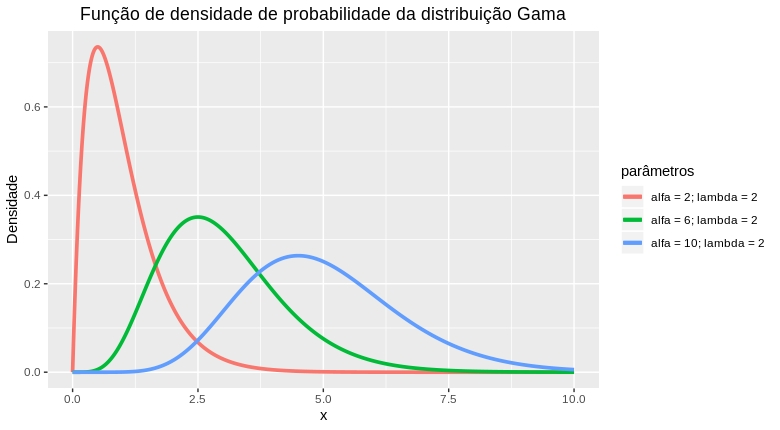
\includegraphics[width = \linewidth]{../../Images/Report_18_10_21/gamma_fixed_lambda.jpeg} 
        }
    \caption{Distribuição Gama}
    \label{fig:gamma}
\end{figure}

\begin{figure}[!h]
    \ContinuedFloat
    \vspace{0.15\linewidth}
    \subfloat[Variação do parâmetro lambda\label{var_lambda:gamma}]{
        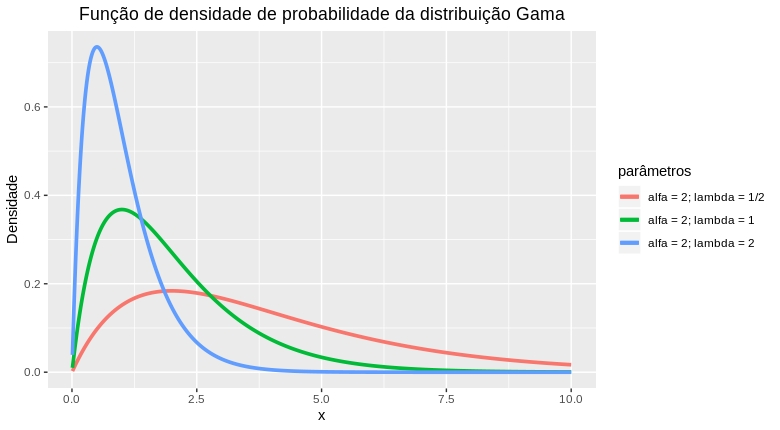
\includegraphics[width = \linewidth]{../../Images/Report_18_10_21/gamma_fixed_alpha.jpeg} 
        }
    \caption{Distribuição Gama}
\end{figure}

\begin{figure}[!h]
    \vspace{0.15\linewidth}
    \subfloat[Variação do parâmetro alfa\label{var_alpha:sqrt_gamma}]{
        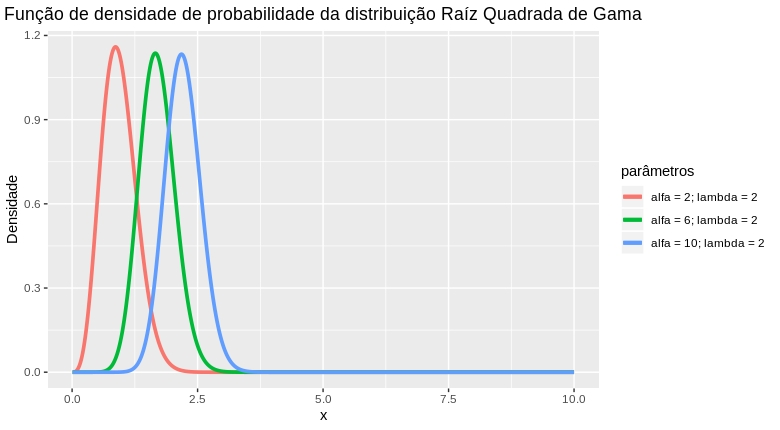
\includegraphics[width = \linewidth]{../../Images/Report_18_10_21/sqrt_gamma_fixed_lambda.jpeg}
    }
    \caption{Distribuição Raíz Quadrada de Gama}
    \label{fig:sqrt_gamma}
\end{figure}

\begin{figure}[!h]
    \ContinuedFloat
    \vspace{0.15\linewidth}
    \subfloat[Variação do parâmetro lambda\label{var_lambda:sqrt_gamma}]{
        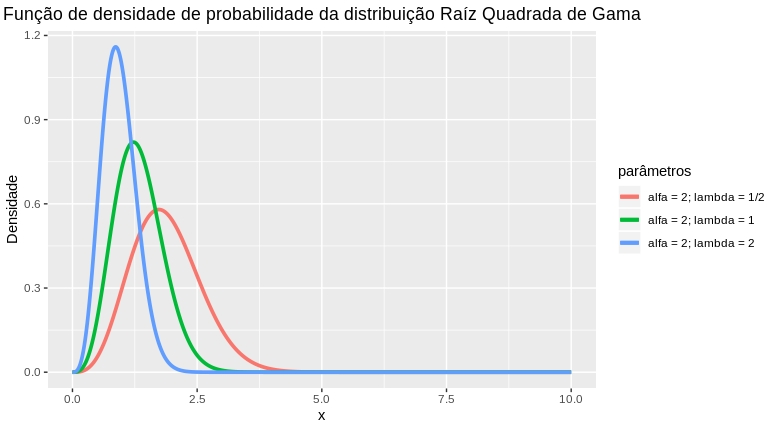
\includegraphics[width = \linewidth]{../../Images/Report_18_10_21/sqrt_gamma_fixed_alpha.jpeg}
    }
    \caption{Distribuição Raíz Quadrada de Gama}
\end{figure}

\begin{figure}[!h]
    \vspace{0.15\linewidth}
    \subfloat[Variação do parâmetro alfa\label{var_alpha:rec_sqrt_gamma}]{
        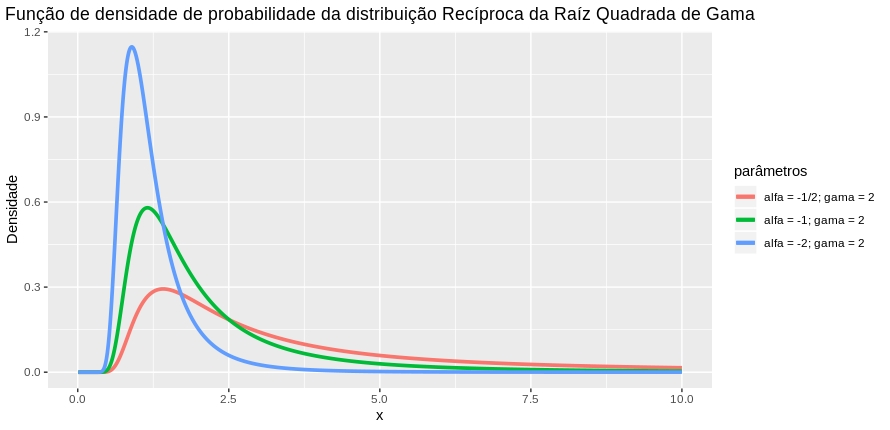
\includegraphics[width = \linewidth]{../../Images/Report_18_10_21/rec_sqrt_gamma_fixed_gamma.jpeg}
    }
    \caption{Distribuição Recíproca da Raíz Quadrada de Gama}
    \label{fig:rec_sqrt_gamma}
    \vspace{0.1\linewidth}
\end{figure}

\begin{figure}[!h]
    \ContinuedFloat
    \vspace{0.15\linewidth}
    \subfloat[Variação do parâmetro gama\label{var_gamma:rec_sqrt_gamma}]{
        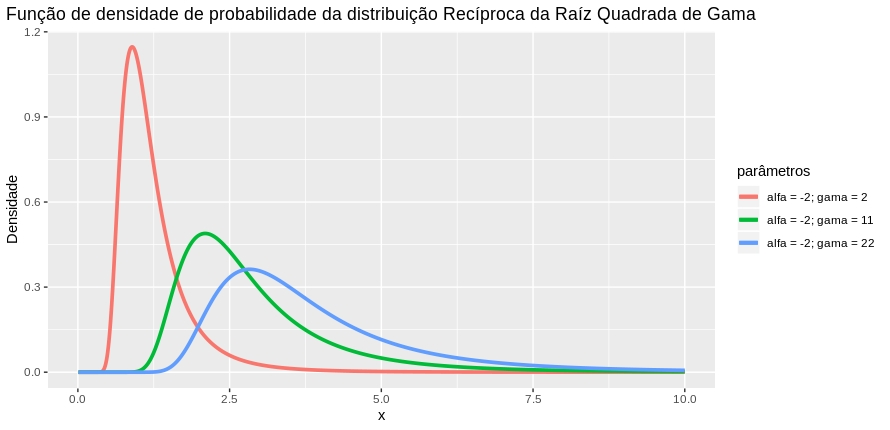
\includegraphics[width = \linewidth]{../../Images/Report_18_10_21/rec_sqrt_gamma_fixed_alpha.jpeg}
    }
    \caption{Distribuição Recíproca da Raíz Quadrada de Gama}
\end{figure}

\begin{figure}[!h]
    \vspace{0.15\linewidth}
    \subfloat[Variação do parâmetro alfa\label{var_alpha:sqrt_gauss}]{
        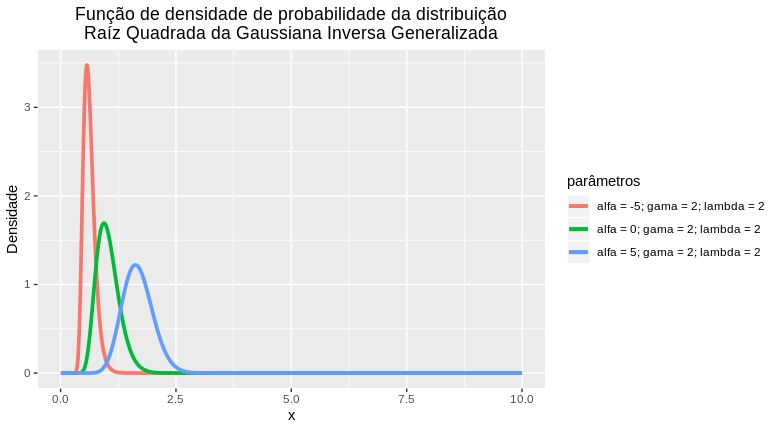
\includegraphics[width = \linewidth]{../../Images/Report_18_10_21/sqrt_gauss_var_alpha.jpeg}
    }
    \caption{Distribuição Raíz Quadrada da Gaussiana Inversa Generalizada}
    \label{fig:sqrt_gauss}
    \vspace{0.1\linewidth}
\end{figure}

\begin{figure}[!h]
    \ContinuedFloat
    \vspace{0.15\linewidth}
    \subfloat[Variação do parâmetro gama\label{var_gamma:sqrt_gauss}]{
        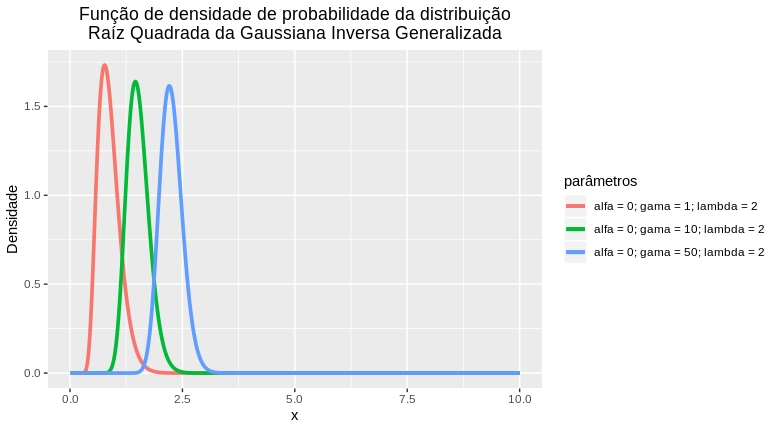
\includegraphics[width = \linewidth]{../../Images/Report_18_10_21/sqrt_gauss_var_gamma.jpeg}
    }
    \caption{Distribuição Raíz Quadrada da Gaussiana Inversa Generalizada}
\end{figure}

\begin{figure}[!h]
    \ContinuedFloat
    \vspace{0.15\linewidth}
    \centering
    \subfloat[Variação do parâmetro lambda\label{var_lambda:sqrt_gauss}]{
        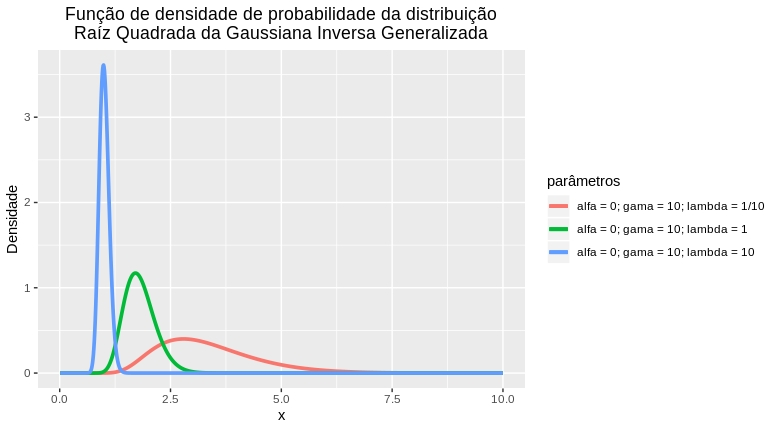
\includegraphics[width = \linewidth]{../../Images/Report_18_10_21/sqrt_gauss_var_lambda.jpeg}
    }
    \caption{Distribuição Raíz Quadrada da Gaussiana Inversa Generalizada}
\end{figure}

\begin{figure}[!h]
    \vspace{0.15\linewidth}
    \subfloat[Variação do parâmetro alfa\label{var_alpha:complex_g}]{
        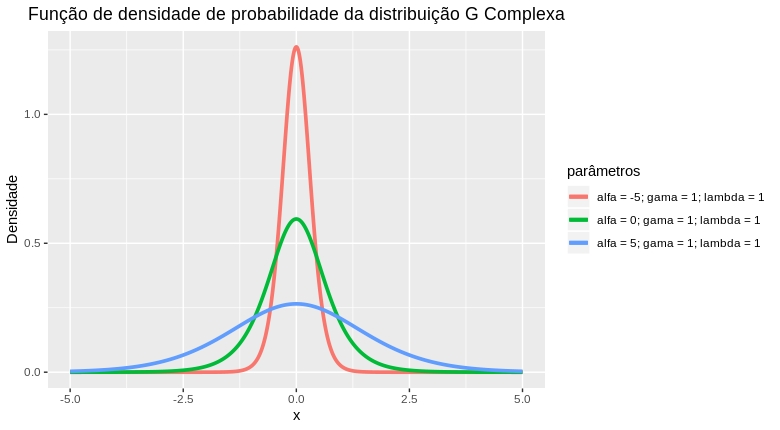
\includegraphics[width = \linewidth]{../../Images/Report_18_10_21/g_c_var_alpha.jpeg}
    }
    \caption{Distribuição G Complexa}
    \label{fig:complex_g}
\end{figure}

\begin{figure}[!h]
    \ContinuedFloat
    \vspace{0.15\linewidth}
    \subfloat[Variação do parâmetro gama\label{var_gamma:complex_g}]{
        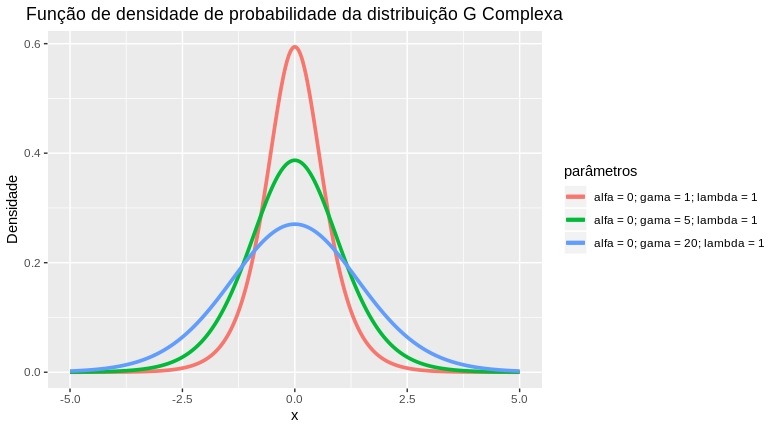
\includegraphics[width = \linewidth]{../../Images/Report_18_10_21/g_c_var_gamma.jpeg}
    }
    \caption{Distribuição G Complexa}
\end{figure}

\begin{figure}[!h]
    \ContinuedFloat 
    \vspace{0.15\linewidth}
    \subfloat[Variação do parâmetro lambda\label{var_lambda:complex_g}]{
        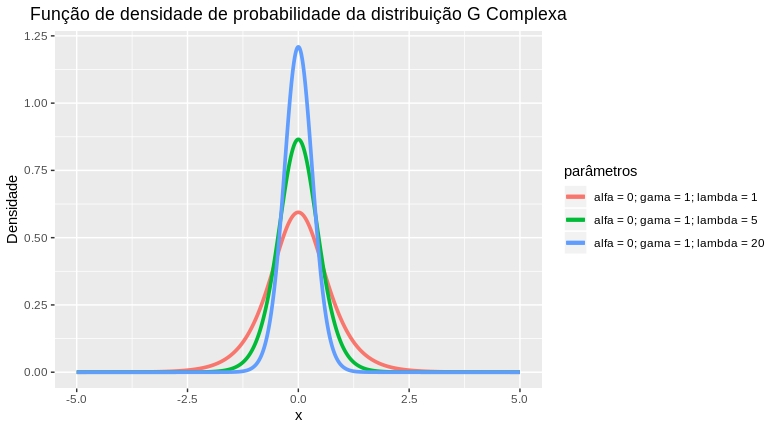
\includegraphics[width = \linewidth]{../../Images/Report_18_10_21/g_c_var_lambda.jpeg}
    }
    \caption{Distribuição G Complexa}
\end{figure}

\begin{figure}[!h]
    \vspace{0.15\linewidth}
    \subfloat[Variação do parâmetro alfa\label{var_alpha:complex_k}]{
        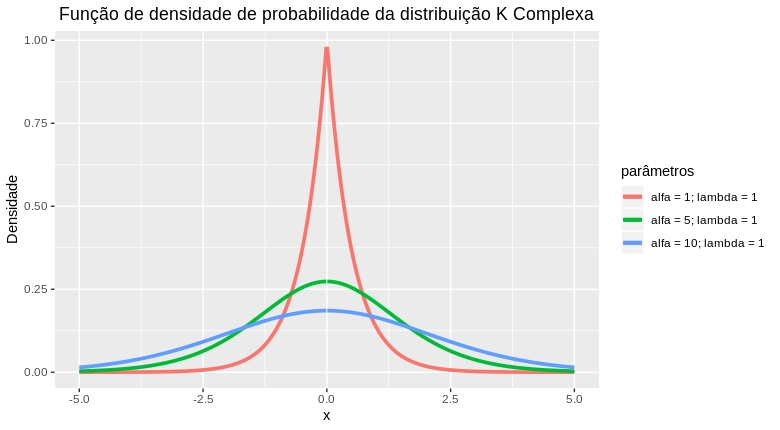
\includegraphics[width = \linewidth]{../../Images/Report_18_10_21/k_c_var_alpha.jpeg}
    }
    \caption{Distribuição K Complexa}
    \label{fig:complex_k}
\end{figure}

\begin{figure}[!h]
    \ContinuedFloat
    \vspace{0.15\linewidth}
    \subfloat[Variação do parâmetro lambda\label{var_lambda:complex_k}]{
        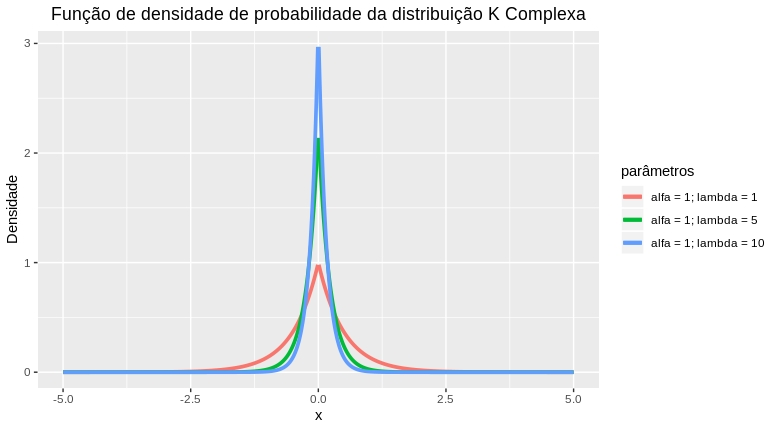
\includegraphics[width = \linewidth]{../../Images/Report_18_10_21/k_c_var_lambda.jpeg}
    }
    \caption{Distribuição K Complexa}
\end{figure}

\begin{figure}[!h]
    \vspace{0.15\linewidth}
    \subfloat[Variação do parâmetro alfa\label{var_alpha:complex_g0}]{
        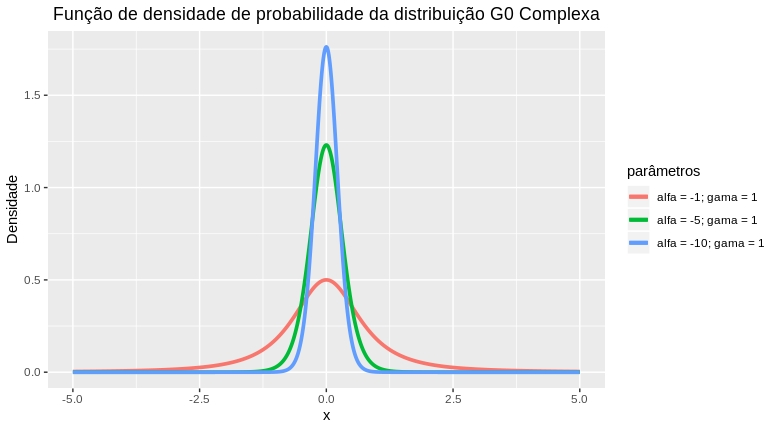
\includegraphics[width = \linewidth]{../../Images/Report_18_10_21/g0_c_var_alpha.jpeg}
    }
    \caption{Distribuição G0 Complexa}
    \label{fig:complex_g0}
\end{figure}

\begin{figure}[!h]
    \ContinuedFloat
    \vspace{0.15\linewidth}
    \subfloat[Variação do parâmetro gama\label{var_gamma:complex_g0}]{
        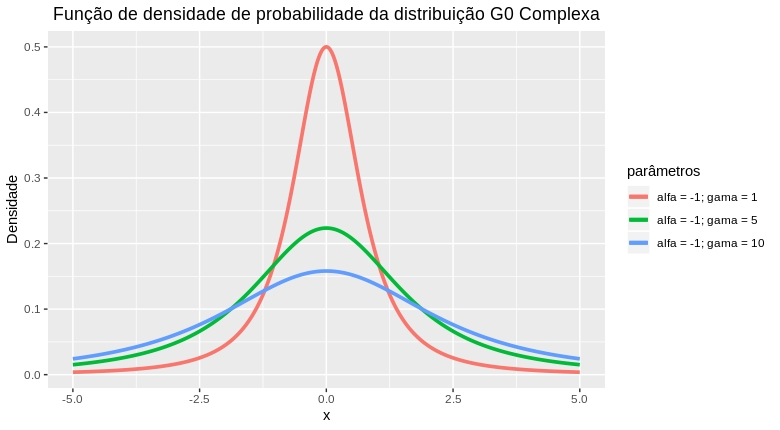
\includegraphics[width = \linewidth]{../../Images/Report_18_10_21/g0_c_var_gamma.jpeg}
    }
    \caption{Distribuição G0 Complexa}
\end{figure}

\begin{figure}[!h]
    \vspace{0.15\linewidth}
    \subfloat[Variação do parâmetro alfa\label{var_alpha:amplitude_g}]{
        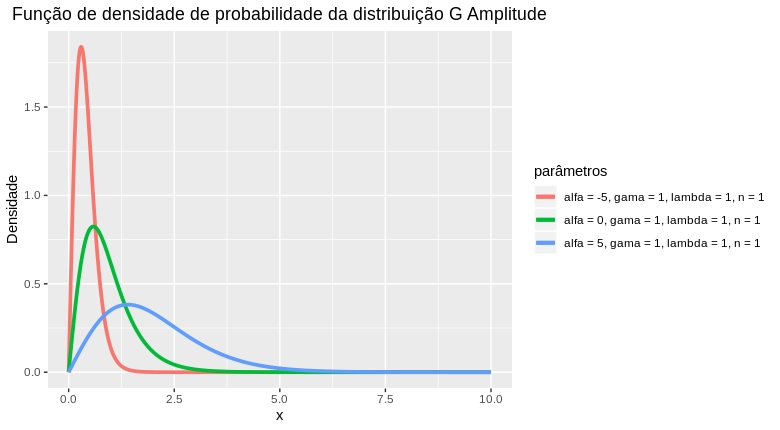
\includegraphics[width = \linewidth]{../../Images/Report_18_10_21/g_a_var_alpha.jpeg}
    }
    \caption{Distribuição G Amplitude}
    \label{fig:amplitude_g}
\end{figure}

\begin{figure}[!h]
    \ContinuedFloat
    \vspace{0.15\linewidth}
    \subfloat[Variação do parâmetro gama\label{var_gamma:amplitude_g}]{
        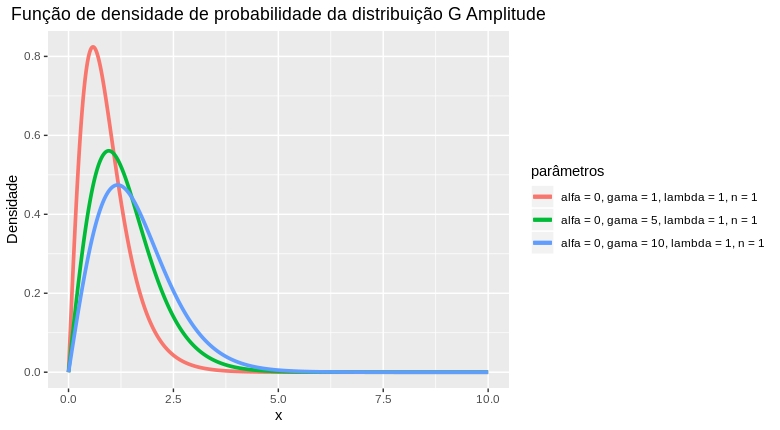
\includegraphics[width = \linewidth]{../../Images/Report_18_10_21/g_a_var_gamma.jpeg}
    }
    \caption{Distribuição G Amplitude}
\end{figure}

\begin{figure}[!h]
    \ContinuedFloat
    \vspace{0.15\linewidth}
    \subfloat[Variação do parâmetro lambda\label{var_lambda:amplitude_g}]{
        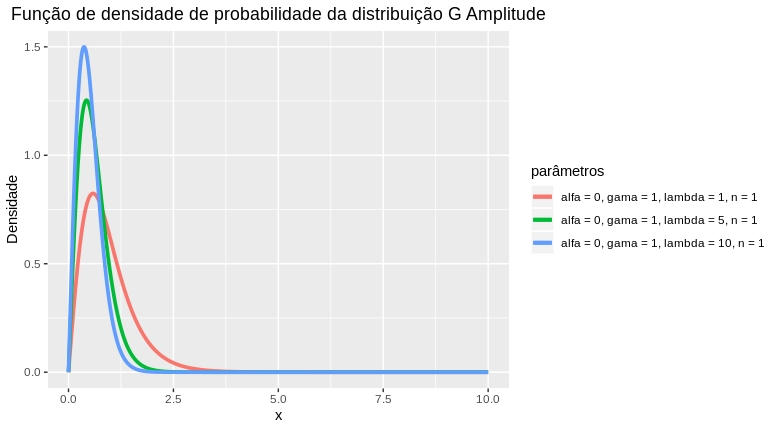
\includegraphics[width = \linewidth]{../../Images/Report_18_10_21/g_a_var_lambda.jpeg}
    }
    \caption{Distribuição G Amplitude}
\end{figure}
    
\begin{figure}[!h]
    \ContinuedFloat
    \vspace{0.15\linewidth}
    \subfloat[Variação do parâmetro n\label{var_n:amplitude_g}]{
        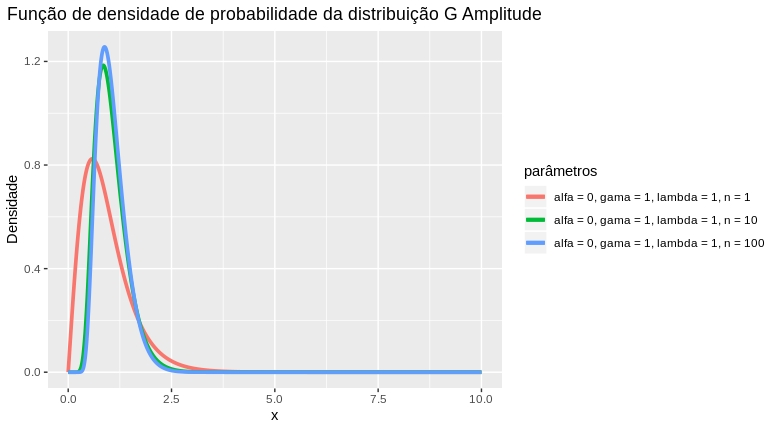
\includegraphics[width = \linewidth]{../../Images/Report_18_10_21/g_a_var_n.jpeg}
    }
    \caption{Distribuição G Amplitude}
\end{figure}

\begin{figure}[!h]
    \vspace{0.15\linewidth}
    \subfloat[Variação do parâmetro alfa\label{var_alpha:amplitude_k}]{
        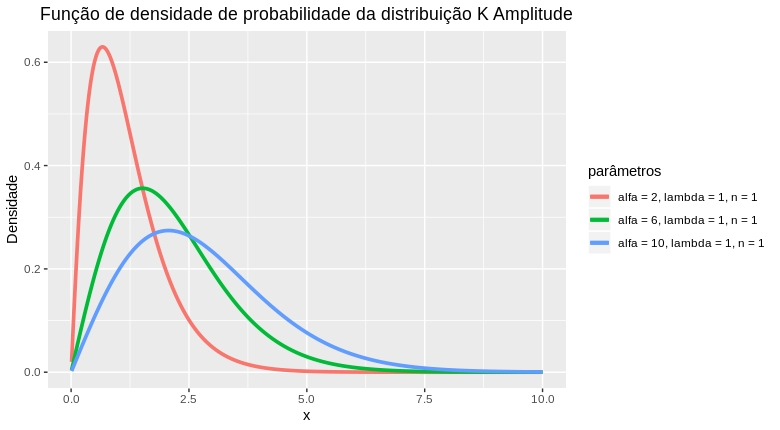
\includegraphics[width = \linewidth]{../../Images/Report_18_10_21/k_a_var_alpha.jpeg}
    }
    \caption{Distribuição K Amplitude}
    \label{fig:amplitude_k}
\end{figure}
    
\begin{figure}[!h]
    \ContinuedFloat
    \vspace{0.15\linewidth}
    \subfloat[Variação do parâmetro lambda\label{var_lambda:amplitude_k}]{
        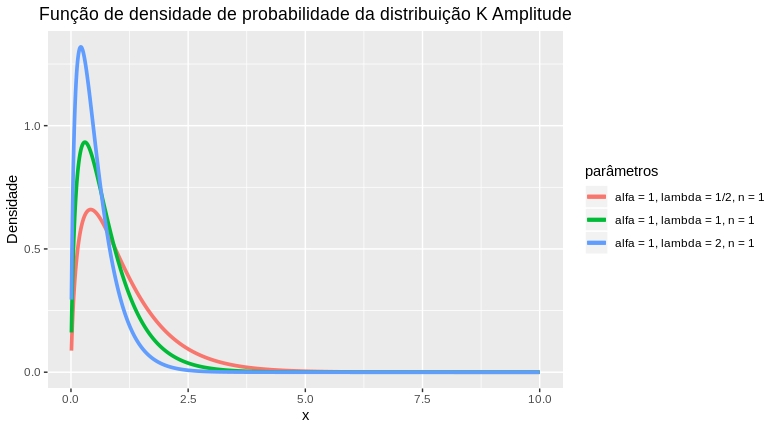
\includegraphics[width = \linewidth]{../../Images/Report_18_10_21/k_a_var_lambda.jpeg}
    }
    \caption{Distribuição K Amplitude}
\end{figure}

\begin{figure}[!h]
    \ContinuedFloat
    \vspace{0.15\linewidth}
    \subfloat[Variação do parâmetro n\label{var_n:amplitude_k}]{
        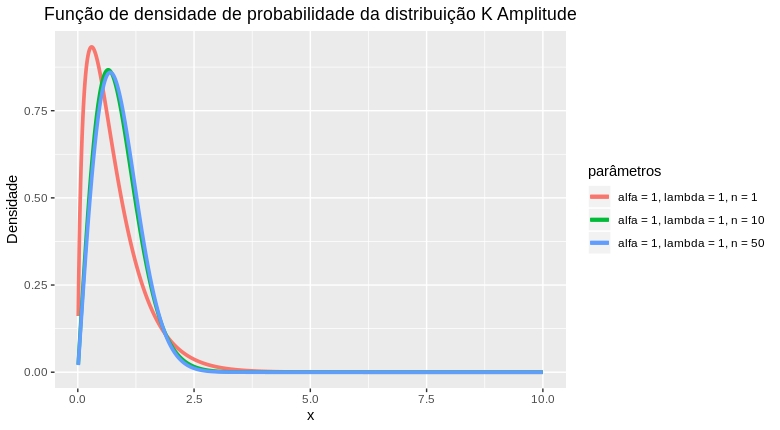
\includegraphics[width = \linewidth]{../../Images/Report_18_10_21/k_a_var_n.jpeg}
    }
    \caption{Distribuição K Amplitude}
\end{figure}

\begin{figure}[!h]
    \vspace{0.15\linewidth}
    \subfloat[Variação do parâmetro alfa\label{var_alpha:amplitude_g0}]{
        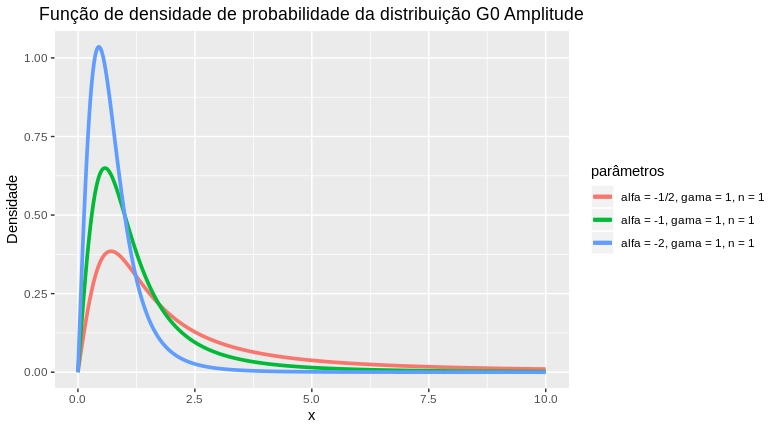
\includegraphics[width = \linewidth]{../../Images/Report_18_10_21/g0_a_var_alpha.jpeg}
    }
    \caption{Distribuição G0 Amplitude}
    \label{fig:amplitude_g0}
\end{figure}

\begin{figure}[!h]
    \ContinuedFloat
    \vspace{0.15\linewidth}
    \subfloat[Variação do parâmetro gama\label{var_gamma:amplitude_g0}]{
        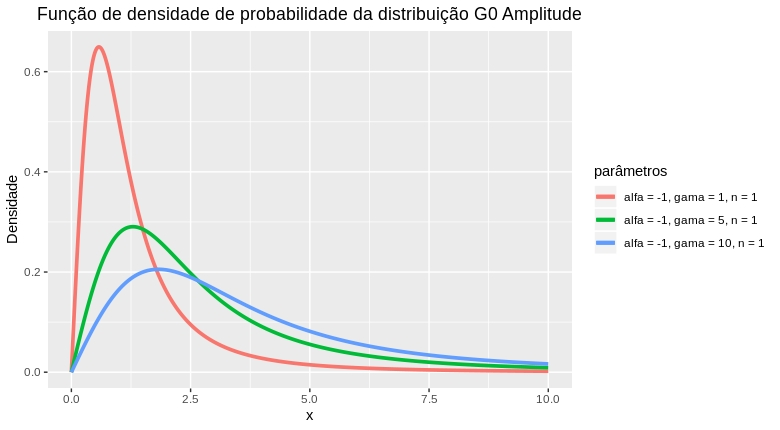
\includegraphics[width = \linewidth]{../../Images/Report_18_10_21/g0_a_var_gamma.jpeg}
    }
    \caption{Distribuição G0 Amplitude}
\end{figure}

\begin{figure}[!h]
    \ContinuedFloat
    \vspace{0.15\linewidth}
    \subfloat[Variação do parâmetro n\label{var_n:amplitude_g0}]{
        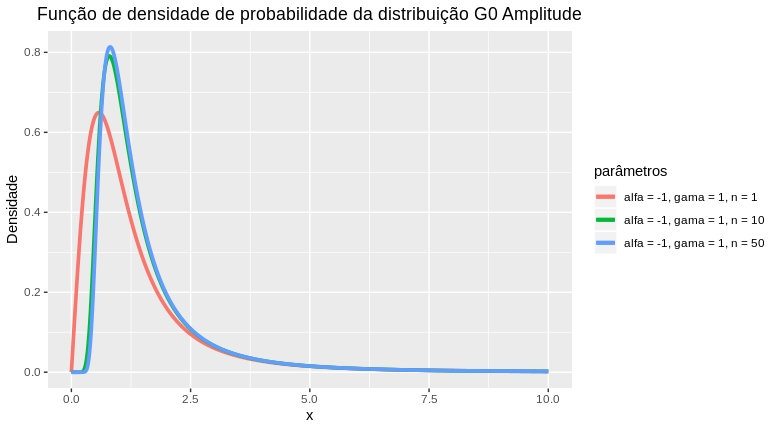
\includegraphics[width = \linewidth]{../../Images/Report_18_10_21/g0_a_var_n.jpeg}
    }
    \caption{Distribuição G0 Amplitude}
\end{figure}

\begin{figure}[!h]
    \vspace{0.15\linewidth}
    \subfloat[Variação do parâmetro alfa\label{var_alpha:intensity_g}]{
        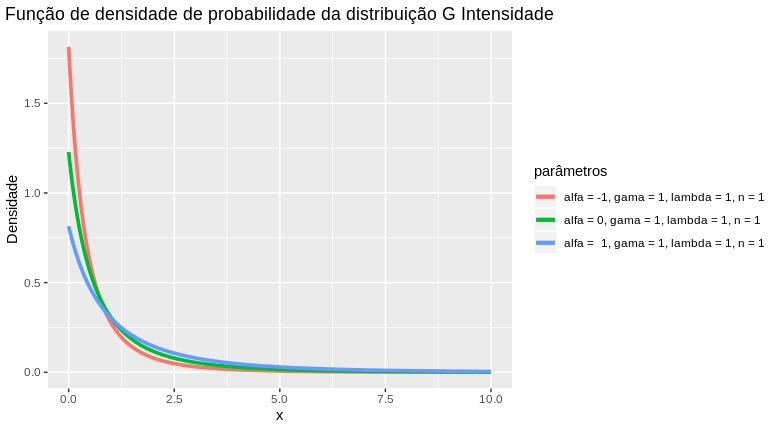
\includegraphics[width = \linewidth]{../../Images/Report_18_10_21/g_i_var_alpha.jpeg}
    }
    \caption{Distribuição G Intensidade}
    \label{fig:intensity_g}
\end{figure}

\begin{figure}[!h]
    \ContinuedFloat
    \vspace{0.15\linewidth}
    \subfloat[Variação do parâmetro gama\label{var_gamma:intensity_g}]{
        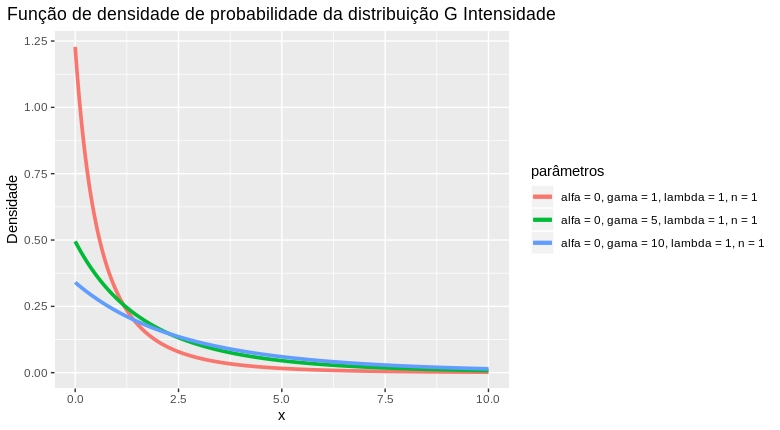
\includegraphics[width = \linewidth]{../../Images/Report_18_10_21/g_i_var_gamma.jpeg}
    }
    \caption{Distribuição G Intensidade}
\end{figure}

\begin{figure}[!h]
    \ContinuedFloat
    \vspace{0.15\linewidth}
    \subfloat[Variação do parâmetro lambda\label{var_lambda:intensity_g}]{
        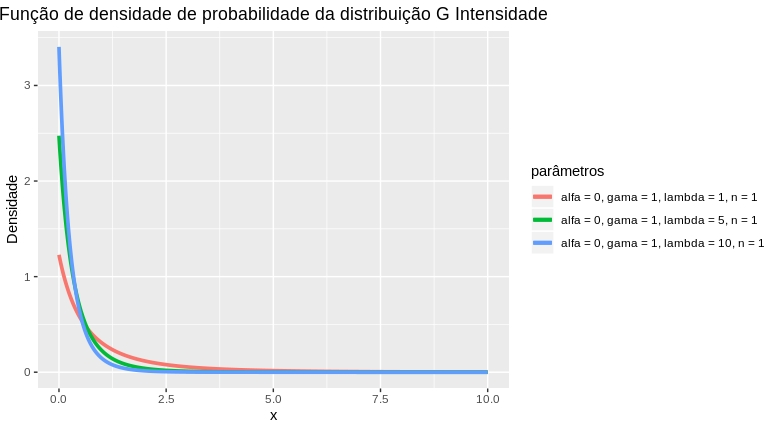
\includegraphics[width = \linewidth]{../../Images/Report_18_10_21/g_i_var_lambda.jpeg}
    }
    \caption{Distribuição G Intensidade}
\end{figure}    

\begin{figure}[!h]
    \ContinuedFloat
    \vspace{0.15\linewidth}
    \subfloat[Variação do parâmetro n\label{var_n:intensity_g}]{
        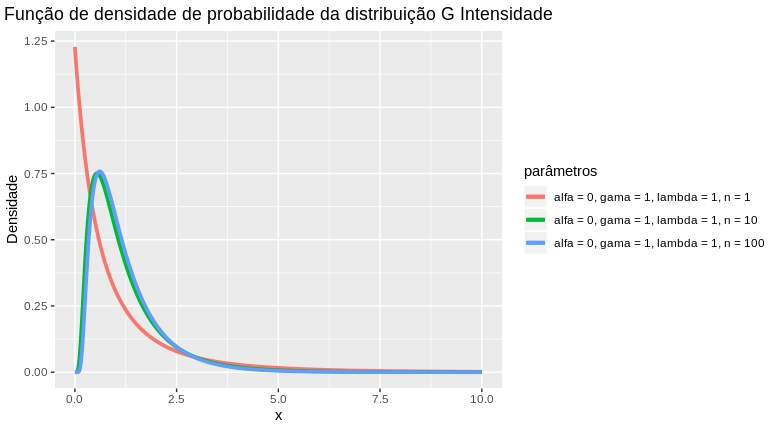
\includegraphics[width = \linewidth]{../../Images/Report_18_10_21/g_i_var_n.jpeg}
    }
    \caption{Distribuição G Intensidade}
\end{figure}

\begin{figure}[!h]
    \vspace{0.15\linewidth}
    \subfloat[Variação do parâmetro alfa\label{var_alpha:intensity_k}]{
        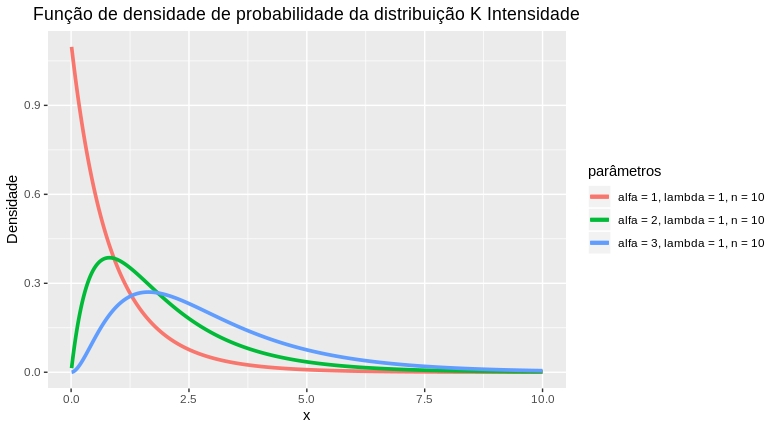
\includegraphics[width = \linewidth]{../../Images/Report_18_10_21/k_i_var_alpha.jpeg}
    }
    \caption{Distribuição K Intensidade}
    \label{fig:intensity_k}
\end{figure}    
 
\begin{figure}[!h]
    \ContinuedFloat
    \vspace{0.15\linewidth}
    \subfloat[Variação do parâmetro lambda\label{var_lambda:intensity_k}]{
        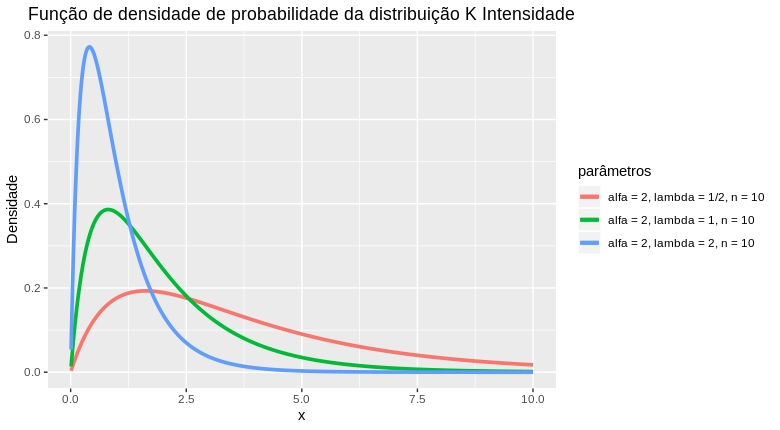
\includegraphics[width = \linewidth]{../../Images/Report_18_10_21/k_i_var_lambda.jpeg}
    }
    \caption{Distribuição K Intensidade}
\end{figure}

\begin{figure}[!h]
    \ContinuedFloat
    \vspace{0.15\linewidth}
    \subfloat[Variação do parâmetro n\label{var_n:intensity_k}]{
        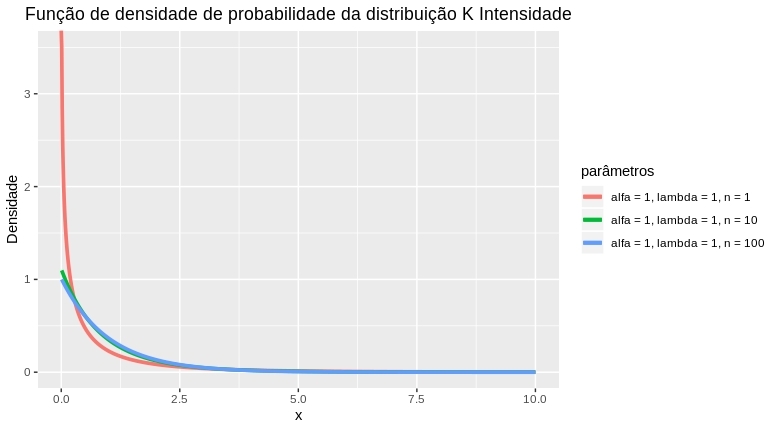
\includegraphics[width = \linewidth]{../../Images/Report_18_10_21/k_i_var_n.jpeg}
    }
    \caption{Distribuição K Intensidade}
\end{figure}

\begin{figure}[!h]
    \vspace{0.15\linewidth}
    \subfloat[Variação do parâmetro alfa\label{var_alpha:intensity_g0}]{
        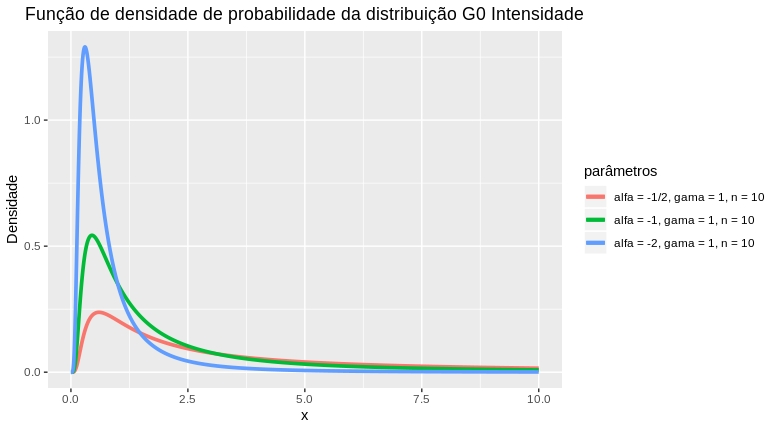
\includegraphics[width = \linewidth]{../../Images/Report_18_10_21/g0_i_var_alpha.jpeg}
    }
    \caption{Distribuição G0 Intensidade}
    \label{fig:intensity_g0}
\end{figure}

\begin{figure}[!h]
    \ContinuedFloat
    \vspace{0.15\linewidth}
    \subfloat[Variação do parâmetro gama\label{var_gamma:intensity_g0}]{
        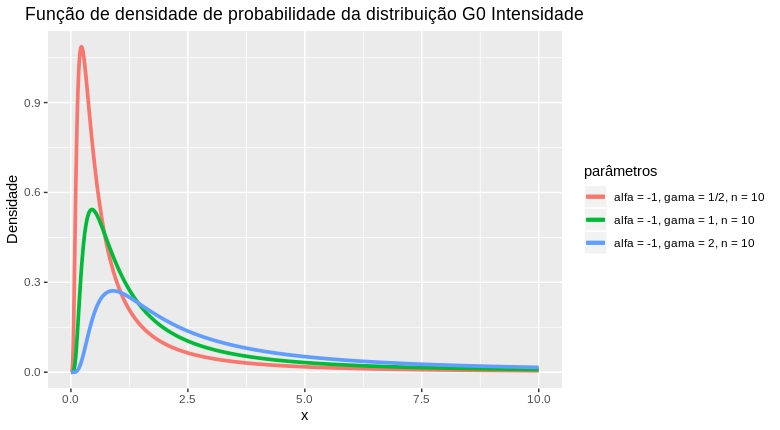
\includegraphics[width = \linewidth]{../../Images/Report_18_10_21/g0_i_var_gamma.jpeg}
    }    
    \caption{Distribuição G0 Intensidade}
\end{figure}

\begin{figure}[!h]
    \ContinuedFloat
    \vspace{0.15\linewidth}
    \subfloat[Variação do parâmetro n\label{var_n:intensity_g0}]{
        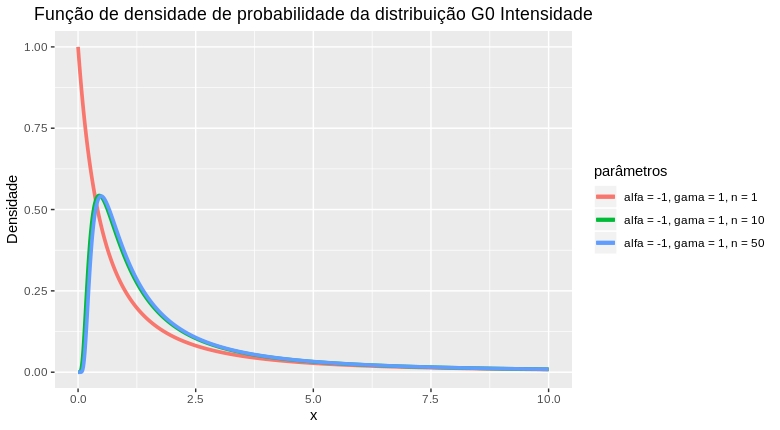
\includegraphics[width = \linewidth]{../../Images/Report_18_10_21/g0_i_var_n.jpeg}
    }
    \caption{Distribuição G0 Intensidade}
\end{figure}

\newpage

\bibliographystyle{abntex2-alf}
\bibliography{../../Bibliography/ref_18_10}
\end{document}



